\documentclass[12pt,a4paper,titlepage]{article}
\usepackage{lab_style}
\usepackage{pdfpages}
\usepackage{eso-pic}
\usepackage{graphicx}
\usepackage{float}
\usepackage{amsmath}

\graphicspath{ {./img/} }
  
\begin{document}

\begin{titlepage}
\selectlanguage{english}

%----------------------------------------------------------------------------------------
% TITLE PAGE INFORMATION
%----------------------------------------------------------------------------------------
  \begin{center} % Center everything on the page

  %----------------------------------------------------------------------------------------
  % HEADING SECTIONS
  %----------------------------------------------------------------------------------------
  \textsc{\large Faculty of Computers, Informatics and Microelectronics}\\[0.5cm]
  \textsc{\large Technical University of Moldova}\\[1.2cm] % Name of your university/college
  \vspace{25 mm}

  \textsc{\Large Object-Oriented Modeling and Analysis}\\[0.5cm] % Major heading such as course name
  \textsc{\large Course Work}\\[0.5cm] % Minor heading such as course title

\newcommand{\HRule}{\rule{\linewidth}{0.5mm}} % Defines a new command for the horizontal lines, change thickness here

  %----------------------------------------------------------------------------------------
  % TITLE SECTION
  %----------------------------------------------------------------------------------------
  \vspace{10 mm}
  \HRule \\[0.4cm]
  { \LARGE \bfseries Analysis and modelling of an online courses platform }\\[0.4cm] % Title of your document
  \HRule \\[1.5cm]

  %----------------------------------------------------------------------------------------
  % AUTHOR SECTION
  %----------------------------------------------------------------------------------------
      \vspace{30mm}

      \begin{minipage}{0.4\textwidth}
      \begin{flushleft} \large
      \emph{Author:}\\
      Cernei \textsc{Liviu}\\
      st. gr. FAF-161
      \end{flushleft}
      \end{minipage}
      ~
      \begin{minipage}{0.4\textwidth}
      \begin{flushright} \large
      \emph{Supervisor:} \\
      Mihail \textsc{Gavrilița}\\ % Supervisor's Name
      university assistant
      \end{flushright}
      \end{minipage}\\[4cm]

      \vspace{5 mm}
      % If you don't want a supervisor, uncomment the two lines below and remove the section above
      %\Large \emph{Author:}\\
      %John \textsc{Smith}\\[3cm] % Your name

      %----------------------------------------------------------------------------------------
      % DATE SECTION
      %----------------------------------------------------------------------------------------

      {\large Chișinau 2018}\\[3cm] % Date, change the \today to a set date if you want to be precise

      %----------------------------------------------------------------------------------------
      % LOGO SECTION
      %----------------------------------------------------------------------------------------

      %\includegraphics{red}\\[0.5cm] % Include a department/university logo - this will require the graphicx package

      %----------------------------------------------------------------------------------------

      \vfill % Fill the rest of the page with whitespace
      \end{center}
      
\end{titlepage}

\cleardoublepage
   \tableofcontents
\newpage

\pagenumbering{arabic}
\setcounter{page}{1}
\setcounter{secnumdepth}{4}

\addtocontents{toc}{\protect\thispagestyle{empty}} % no page number on the table of contents page
\cleardoublepage


\phantomsection
\addcontentsline{toc}{section}{Introduction}

\section{Intro and Theory}
\subsection{Project Description, User Stories}
The new \textbf{St. Courses} platform is a great place to learn new skills and boost your knowledge. It provides a web based interaction between students and teachers. Because of it's simplicity and security, it can be used by schools and universities. On St. Courses, the user gets personalized help in order to customize his online classes.
The website is user-friendly, engaging and easy to use. It also has a customizable front-end, advanced analytics and much more.

The platform is populated by 3 kinds of actors: administrators, teachers and students.

\textbf{Courses:}
A course has a title, description and content. It is placed in time by the start date and end date. It is created by a teacher and can have enroled students.
The content is structured in chapters and can contain text, images and interactive elements.
Every teacher who logged in can create and edit a course. To delete it, he must complete a request to an administrator, containing the cause of removal.

\textbf{Tests:}
The teacher optionally can create a test to evaluate the quality of the course. For this he must fill in the questions, provide the coorect answers and create an grading system.
For the student, a test is obligatory. At the end of the course the students get marks based on their activity.

\textbf{Feedback:}
Both teachers and students can give feedback which wil be assigned to the course history.

\textbf{Enrolment to a course:}
The courses are free, meaning that everyone with an account can enrol to any corse. However, there are recomended courses, based on age, fields of interest, difficulty level.
A student can lose access to a course if he unenroled himself, or the teacher removed him.
In both cases the student loses the progress, tests, marks gained in that course.

\textbf{Invitations:}
A teacher can send invitations to a course. The invited students will be enroled automatically. With this method the teacher can assemble an real-life grop and assure access to the course for them.

\begin{itemize}
	\item
	An administrator (moderator) is responsible for handling reports, managing courser and users..
	\item 
	A teacher can create a new course, edit an existing one, approve or reject an student to a course, create tests.
	\item
	A student can enrol to a course, read the material, unenrol from a course, pass a test, give feedback.
\end{itemize}

\subsection{Modeling Languages}
A modeling language is any artificial language that can be used to express information or knowledge or systems in a structure that is defined by a consistent set of rules. The rules are used for interpretation of the meaning of components in the structure.\par
A modeling language can be graphical or textual.\par
\textbf{Graphical} modeling languages use a diagram technique with named symbols that represent concepts and lines that connect the symbols and represent relationships and various other graphical notation to represent constraints.\par
\textbf{Textual} modeling languages may use standardized keywords accompanied by parameters or natural language terms and phrases to make computer-interpretable expressions.\par
Not all modeling languages are executable, and for those that are, the use of them doesn't necessarily mean that programmers are no longer required. On the contrary, executable modeling languages are intended to amplify the productivity of skilled programmers, so that they can address more challenging problems, such as parallel computing and distributed systems.\par

\subsection{Conceptual OO Analysis / Technical OO Design}
\textbf{Object-Oriented Analysis}
\begin{itemize}  
	\item Elicit requirements: Define what does the software need to do, and what’s the problem the software trying to solve.
	\item Specify requirements: Describe the requirements, usually, using use cases (and scenarios) or user stories.
	\item Conceptual model: Identify the important objects, refine them, and define their relationships and behavior and draw them in a simple diagram.
\end{itemize}
\textbf{Conceptual Model}
\begin{itemize}  
	\item Identifying Objects
	\item Refining Objects
	\item Drawing Objects
	\item Identifying Object Relationships
	\item Identifying Object Behaviors
\end{itemize}


\subsection{Abstraction, Encapsulation, Decomposition, Generalization}
Most modern programming languages support and encourage object-oriented programming (OOP). It's main principles are:\par \textbf{Abstraction} is the idea of simplifying a concept to its bare essentials in some context. It allows you to better understand the concept by stripping it down to a simplified version.\par \textbf{Encapsulation} can be thought of as putting something inside a capsule - you limit its exposure to the outside world. In software, restricting access to inner objects and properties helps with data integrity.\par \textbf{Decomposition} is the action of splitting an object into multiple separate smaller parts. Said parts are easier to understand, maintain and program.\par \textbf{Generalization} might be the most important design principle - it is the process of extracting shared characteristics and combining them in one place. All of us know about the concept of functions and class inheritance —both are a kind of generalization.\par

\subsection{Coupling and Cohesion, Separation of Concerns, Information Hiding, Conceptual integrity}
\textbf{Coupling} - An indication of the strength of interconnections between program units.
Highly coupled have program units dependent on each other. Loosely coupled are made up of units that are independent or almost independent.\par

\textbf{Cohesion} - Measure of how well module fits together.
A component should implement a single logical function or single logical entity. All the parts should contribute to the implementation.\par
\textbf{Separation of Concerns} (SoC) is a design principle for separating a computer program into distinct sections, such that each section addresses a separate concern. A concern is a set of information that affects the code of a computer program. A concern can be as general as the details of the hardware the code is being optimized for, or as specific as the name of a class to instantiate. A program that embodies SoC well is called a modular program. Modularity, and hence separation of concerns, is achieved by encapsulating information inside a section of code that has a well-defined interface. Encapsulation is a means of \textbf{information hiding}. Layered designs in information systems are another embodiment of separation of concerns (e.g., presentation layer, business logic layer, data access layer, persistence layer).\par
\textbf{Conceptual integrity} is the principle that anywhere you look in your system, you can tell that the design is part of the same overall design. This includes low-level issues such as formatting and identifier naming, but also issues such as how modules and classes are designed, etc.\par
\subsection{Solid / Grasp Principles}
\textbf{SOLID Principles are principles of class design.}
\begin{itemize}
	\item SRP: Single Responsibility Principle–An object should have only a single responsibility and all the responsibility should be entirely encapsulated by the class.–There should never be more than one reason for a class to change
	\item OCP: Open/Closed Principle–Software entities should be open for extension, but closed for modification
	\item LSP: Liskov Substituion Principle–Objects in a program should be replaceable with instances of their subtypes without altering the correctness of that program
	\item ISP: Interface Segregation Principle–many client specific interfaces are better than one general purpose interface–once an interface has gotten too 'fat' split it into smaller and more specific interfaces so that any clients of the interface will only know about the methods that pertain to them. No client should be forced to depend on methods it does not use
	\item DIP: Dependency Inversion Principle–Depend upon Abstractions. Do not depend upon concretions.Dependency Injection (DI) is one method of following this principle.
\end{itemize}

\textbf{GRASP - Acronym for General Responsibility Assignment Software Patterns.}
\begin{itemize}
	\item Assigning responsibilities to classes is a critical aspect of object-oriented design.
	\item Appropriate assignment of responsibilities to classes is the key to successful design.
	\item There are fundamental principles in assigning responsibilities that experienced designers apply.
	\item These principles are summarized in the GRASP patterns.
	\item Has nine core principles that object-oriented designers apply when assigning responsibilities to classes and designing message interactions.
\end{itemize}

\subsection{Software Development Process}
In software engineering, a \textbf{software development process} is the process of dividing software development work into distinct phases to improve design, product management, and project management. It is also known as a software development life cycle. The methodology may include the pre-definition of specific deliverables and artifacts that are created and completed by a project team to develop or maintain an application.\par
Most modern development processes can be vaguely described as agile. Other methodologies include waterfall, prototyping, iterative and incremental development, spiral development, rapid application development, and extreme programming.\par
\subsection{Top-down and Bottom-up Design}
Top-down and bottom-up are both strategies of information processing and knowledge ordering, used in a variety of fields including software, humanistic and scientific theories (see systemics), and management and organization. In practice, they can be seen as a style of thinking, teaching, or leadership.\par
A \textbf{top-down} approach (also known as stepwise design and in some cases used as a synonym of decomposition) is essentially the breaking down of a system to gain insight into its compositional sub-systems in a reverse engineering fashion. In a top-down approach an overview of the system is formulated, specifying, but not detailing, any first-level subsystems. Each subsystem is then refined in yet greater detail, sometimes in many additional subsystem levels, until the entire specification is reduced to base elements. A top-down model is often specified with the assistance of "black boxes", which makes it easier to manipulate. However, black boxes may fail to clarify elementary mechanisms or be detailed enough to realistically validate the model. Top down approach starts with the big picture. It breaks down from there into smaller segments.\par
A \textbf{bottom-up} approach is the piecing together of systems to give rise to more complex systems, thus making the original systems sub-systems of the emergent system. Bottom-up processing is a type of information processing based on incoming data from the environment to form a perception. From a cognitive psychology perspective, information enters the eyes in one direction (sensory input, or the "bottom"), and is then turned into an image by the brain that can be interpreted and recognized as a perception (output that is "built up" from processing to final cognition). In a bottom-up approach the individual base elements of the system are first specified in great detail. These elements are then linked together to form larger subsystems, which then in turn are linked, sometimes in many levels, until a complete top-level system is formed. This strategy often resembles a "seed" model, by which the beginnings are small but eventually grow in complexity and completeness. However, "organic strategies" may result in a tangle of elements and subsystems, developed in isolation and subject to local optimization as opposed to meeting a global purpose.\par

\subsection{OntoUML}
\textbf{OntoUML} is a pattern-based and ontologically well-founded version of the Unified Modeling Language (UML). Its meta-model has been designed in compliance with the ontological distinctions of a well-grounded theory, named the Unified Foundational Ontology (UFO). OntoUML includes a system of interrelated axiomatic theories, providing modeling foundations for all Conceptual Modeling major concepts, including theories for: types and taxonomic structures (including roles), part-whole relations, events, formal and material relations, dependent (weak) entities, attributes and attribute value and measurement spaces (roughly datatypes). \par


\section{Analysis and Modeling}
\subsection{Main and Alternative Flows}
\begin{itemize}
\item
\noindent\textbf{Student Use Case diagram - Enrol in course}
\begin{description}
    \item[Success scenario:]
\end{description}
\renewcommand{\labelenumii}{\arabic{enumii}}
\begin{itemize}
  \item 1. The student navigates to "Courses" page
  \item 2. The student selects from the list a course
  \item 3. The student clicks the [Enrol] button.
  \item 4. The system outputs success message.
\end{itemize}
\begin{description}
    \item[Alternate flow:]
\end{description}
\begin{itemize}
  \item 1.a The student is enroled to the course by a teacher, other steps are not performed.
  \item 2.a The student inputs name of course in the search box
\end{itemize}
\item
\noindent\textbf{Teacher Use Case diagram - Create course}
\begin{description}
    \item[Success scenario:]
\end{description}
\renewcommand{\labelenumii}{\arabic{enumii}}
\begin{itemize}
  \item 1. The teacher navigates to "Courses" page
  \item 2. The teacher clicks the [New] button.
  \item 3. The teacher writes the title, date, content.
  \item 4. The teacher clicks the [Save] button.
  \item 5. The system outputs success message.
\end{itemize}
\begin{description}
    \item[Alternate flow:]
\end{description}
\begin{itemize}
  \item 3.a The teacher writes the title, date and imports the pdf file with the content.
\end{itemize}

\item
\noindent\textbf{Admin Use Case diagram - Login}
\begin{description}
    \item[Success scenario:]
\end{description}
\renewcommand{\labelenumii}{\arabic{enumii}}
\begin{itemize}
  \item 1. The admin navigates to "Login" page
  \item 2. The admin inputs correct username and correct password.
  \item 3. The admin clicks the [Login] button.
  \item 4. The system outputs success message.
\end{itemize}
\begin{description}
    \item[Alternate flow:]
\end{description}
\begin{itemize}
  \item 2.a The admin inputs wrong username or wrong password, fails to login but attempts one more time with correct username and correct password.
  \item 3.a The admin presses the [Enter] key on the keyboard.
\end{itemize}
\end{itemize}

\subsection{Requirements}
\noindent\textbf{Functional}
\begin{itemize}
	\item Provide access to intersting courses
	\item Teachers can create new courses
	\item Students can take tests
	\item Students can give feedback
	\item Teachers can invite and enroll students
\end{itemize}
\textbf{Non-Functional}
\begin{itemize}
	\item The site supports multiple users at the same time
	\item The information is stored and encripted safely
	\item The site provides very fast access to data
	\item The site can provides access in multiple countries.
	\item The information is processed real-time.
\end{itemize}

\subsection{Technologies}
\textbf{Model–view–controller} is commonly used for developing software that divides an application into three interconnected parts. This is done to separate internal representations of information from the ways information is presented to and accepted from the user. The MVC design pattern decouples these major components allowing for efficient code reuse and parallel development.\par
Traditionally used for desktop graphical user interfaces (GUIs), this architecture has become popular for designing web applications and even mobile, desktop and other clients. Popular programming languages like Java, C\#, Ruby, PHP and others have popular MVC frameworks that are currently being used in web application development straight out of the box.\par

\subsection{SWOT Analysis}
\noindent\textbf{Strengths}
\begin{itemize}
	\item Customer-centric design and messaging
	\item Useful and relevant content
	\item Intuitive navigation and search
	\item Quick and easy enrollment process
	\item Responsive design with full mobile support
\end{itemize}
\textbf{Weaknesses}
\begin{itemize}
	\item The lack of a content specialist within the web team.
	\item Minor updates and not thinking strategically.
	\item Limitations over the type of content published
\end{itemize}
\textbf{Opportunities}
\begin{itemize}
	\item New technologies to improve user experience
	\item Emerging new and untapped markets
	\item New niches and market segments
	\item New design trends to better convey messages
	\item More effective marketing tactics
	\item Positive changes in social factors
\end{itemize}
\textbf{Threats}
\begin{itemize}
	\item Competitors copying features or ideas
	\item Emergence of new competitors
	\item Changing customer needs
	\item New laws or regulations
	\item SPAM \& unsolicited advertising
	\item Upgraded browser software
\end{itemize}

\subsection{Domain Analysis}
\textbf{Online courses} are aimed at unlimited participation and open access via the web. In addition to traditional course materials such as filmed lectures, readings, and problem sets, many online courses provide interactive user forums to support community interactions among students, professors, and teaching assistants (TAs).\par
Online courses are regarded by many as an important tool to widen access to Higher Education (HE) for millions of people, including those in the developing world, and ultimately enhance their quality of life. Online courses may be regarded as contributing to the democratisation of HE, not only locally or regionally but globally as well. Online courses can help democratise content and make knowledge reachable for everyone. Students are able to access complete courses offered by universities all over the world, something previously unattainable. With the availability of affordable technologies, online courses increase access to an extraordinary number of courses offered by world-renowned institutions and teachers.\par
There are already similar platforms. \textbf{"Coursera"} emerged as the top ranked online courses platform and the best overall choice due to its impressive selection of learning pathways and course features. \textbf{"edX"} and \textbf{"Udacity"} were also found to be strong contenders.

\subsection{Project Setup. Delivery / Installation Documentation}
The last step of website development is \textbf{deployment}. The process of“getting your website on the web” consists of a number of steps:
\begin{itemize}
\item Finding a domain name
\item Finding a hosting service
\item Uploading files with SFTP
\item Deploying server-side applications
\end{itemize}
But the client is not required to download or install anything. He simply navigates to the webpage. The only step he should take is to create an account.

\section{Analysis and Modeling in UML}
\subsection{Use Case Diagram}
In Figure ~\ref{fig:2student} is represented the Use Case diagram for the actor "student".
\begin{figure}[H]
\centering
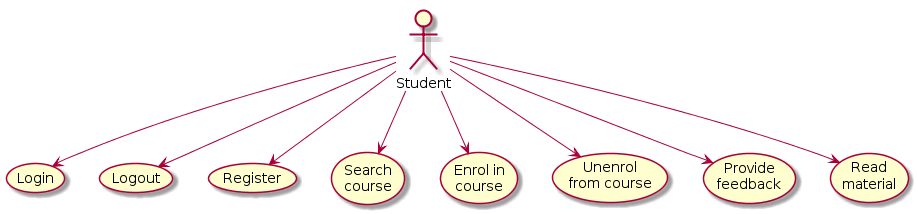
\includegraphics[width=\textwidth]{2student}
\caption{Student Use Case diagram}
\label{fig:2student}
\end{figure}

In order to be able to login the student should have an account. Also, to logout the student should firstly login. Another case is the registration - the student must provide personal information (first / last name, year of study, university, faculty. group etc.). After registration, the user searches a course, the student can input the name of teacher or the title of the lecture.\par
Enrolment in a course is performed by selecting a course, clicking the [Enrol] button and accepting the confirmation message. The same with the unenrollment procedure.
Finally, the student selects a course in which he is already enroled and can start reading the content.
At the bottom of the page the student also can find the "Feedback" form.
\clearpage

In Figure ~\ref{fig:2teacher} is represented the Use Case diagram for the actor "teacher".
\begin{figure}[H]
\centering
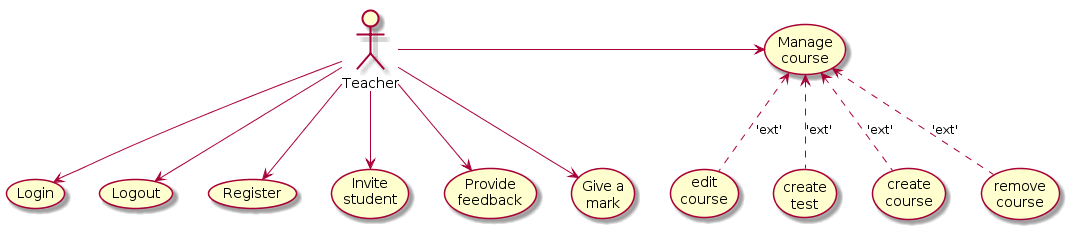
\includegraphics[width=\textwidth]{2teacher}
\caption{Teacher Use Case diagram}
\label{fig:2teacher}
\end{figure}
The teacher has access like the student user, but with additional privileges. He invite a student to one of his own courses. The teacher is responsible for giving marks or evaluating the student at the end of course.\par
Also, the techer is in control of the content of the course - we can say that he can perform "CRUD" operations on his own courses.

In Figure ~\ref{fig:2admin} is represented the Use Case diagram for the actor "administrator".
\begin{figure}[H]
\centering
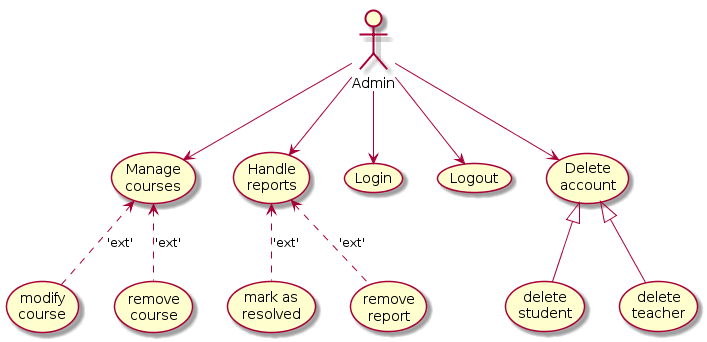
\includegraphics[width=\textwidth]{2admin}
\caption{Admin Use Case diagram}
\label{fig:2admin}
\end{figure}

The administrator can do almost everything he wants. He can manage courses from any teacher, can remove any accounts. Also he is responsible for handling reports.

\subsection{Sequence Diagram}
In Figure ~\ref{fig:3login} is represented the sequence diagram for the login operation.
\begin{figure}[H]
	\centering
	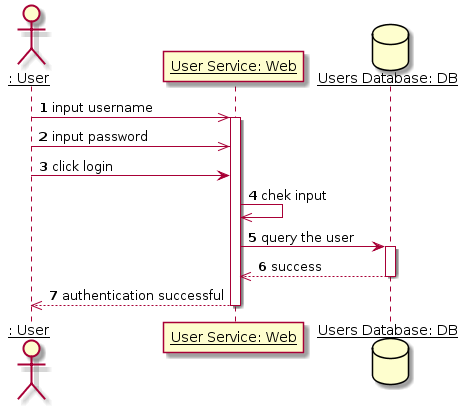
\includegraphics[width=15cm]{3login}
	\caption{Login sequence diagram}
	\label{fig:3login}
\end{figure}
We observe the sequence of operations needed to login any user: student, teacher, or even admin. It is a generalized operation, thats why I used an anonymous calss. The user inputs username and password, the user service check it and sends the information further to the database. The database returns an "success" message, which is propagated to the user by the service. This is the case when all information was correct, and results with the user authenticated.\par

In Figure ~\ref{fig:3create} is represented the sequence diagram for creation of a new course.
\begin{figure}[H]
	\centering
	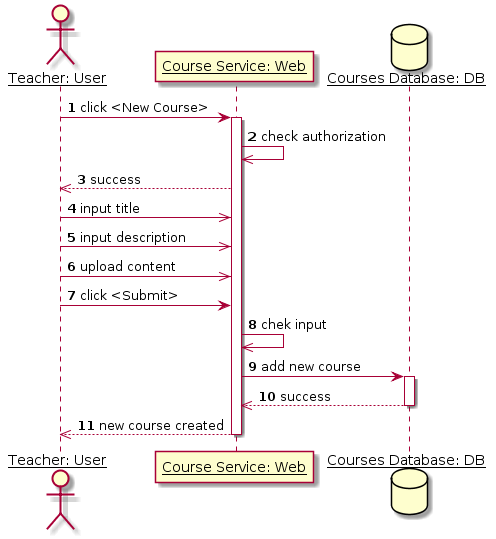
\includegraphics[width=15cm]{3create}
	\caption{New course sequence diagram}
	\label{fig:3create}
\end{figure}
This diagram is specifically for the teacher. In order to create a course, the teacher should have assignet a special authorization key. If it is found, he can begin to input the course information. When submitted, it is checked for invalid fields, then it is sent to the course database. In case of success the teacher is announced through the course service.

In Figure ~\ref{fig:3feedback} is represented the sequence diagram for giving feedback for a course.
\begin{figure}[H]
\centering
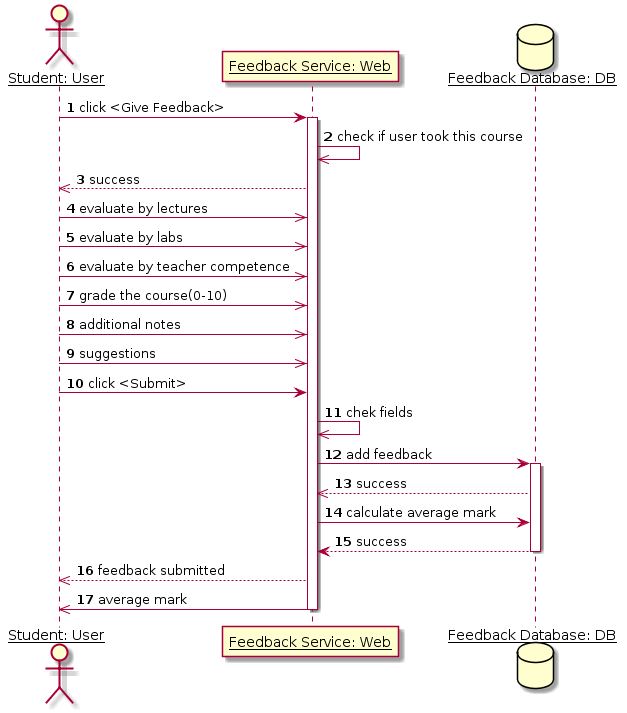
\includegraphics[width=15cm]{3feedback}
\caption{Feedback sequence diagram}
\label{fig:3feedback}
\end{figure}
To be eligible to give feedback, the studnt should have already completed the course. If the condition is satisfied, he can fill the form. After submission, all fields are checked and the information is sent to the database. After a "success" message, the feedback service requests the average mark for that course. Then the student receives an acceptance message and can see the overall quality of the course.

\subsection{Collaboration Diagram}
In Figure ~\ref{fig:4login} is represented the collaboration diagram for the login operation.
\begin{figure}[H]
\centering
	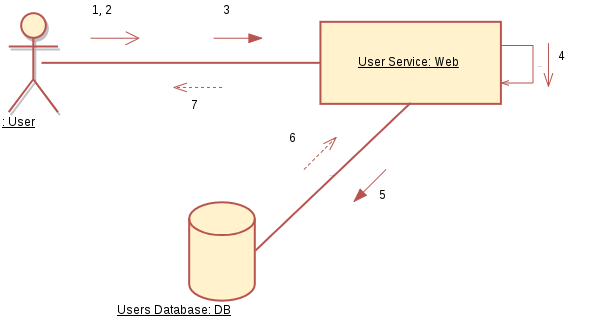
\includegraphics[width=15cm]{4login}
	\caption{Login collaboration diagram}
	\label{fig:4login}
\end{figure}
Here we can see the interaction beween objects in our project. These diagrams are the equivalent of the previous sequence diagrams.\par
\noindent 1 - input username;
2 - input password;
3 - click login;
4 - chek input;
5 - query the user;
6 - success;
7 - authentication successful;

In Figure ~\ref{fig:4create} is represented the collaboration diagram for creation of a new course.
\begin{figure}[H]
\centering
	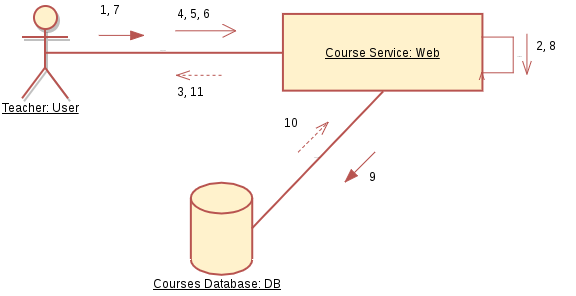
\includegraphics[width=15cm]{4create}
	\caption{New course collaboration diagram}
	\label{fig:4create}
\end{figure}
\noindent 1 - click [New Course];
 2 - check authorization;
 3 - success;
 4 - input title;
 5 - input description;
 6 - upload content;
 7 - click [Submit];
 8 - chek input;
 9 - add new course;
10 - success;
11 - new course created;

In Figure ~\ref{fig:4feedback} is represented the collaboration diagram for giving feedback for a course.
\begin{figure}[H]
\centering
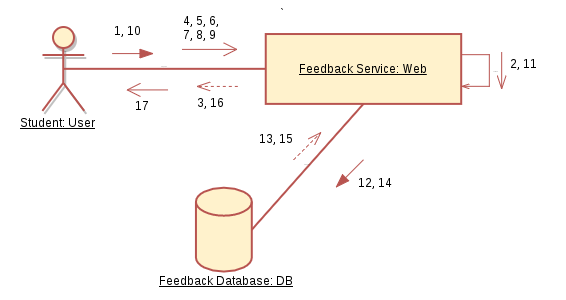
\includegraphics[width=15cm]{4feedback}
\caption{Feedback collaboration diagram}
\label{fig:4feedback}
\end{figure}
\noindent 1 - click [Give Feedback];
 2 - check if user took this course;
 3 - success;
 4 - evaluate by lectures;
 5 - evaluate by labs;
 6 - evaluate by teacher competence;
 7 - grade the course(0-10);
 8 - additional notes;
 9 - suggestions;
10 - click [Submit];
11 - chek fields;
12 - add feedback;
13 - success;
14 - calculate average mark;
15 - success;
16 - feedback submitted;
17 - average mark;

\subsection{Class Diagram}
In Figure ~\ref{fig:5class} is represented the class diagram for the website.
\begin{figure}[H]
	\centering
	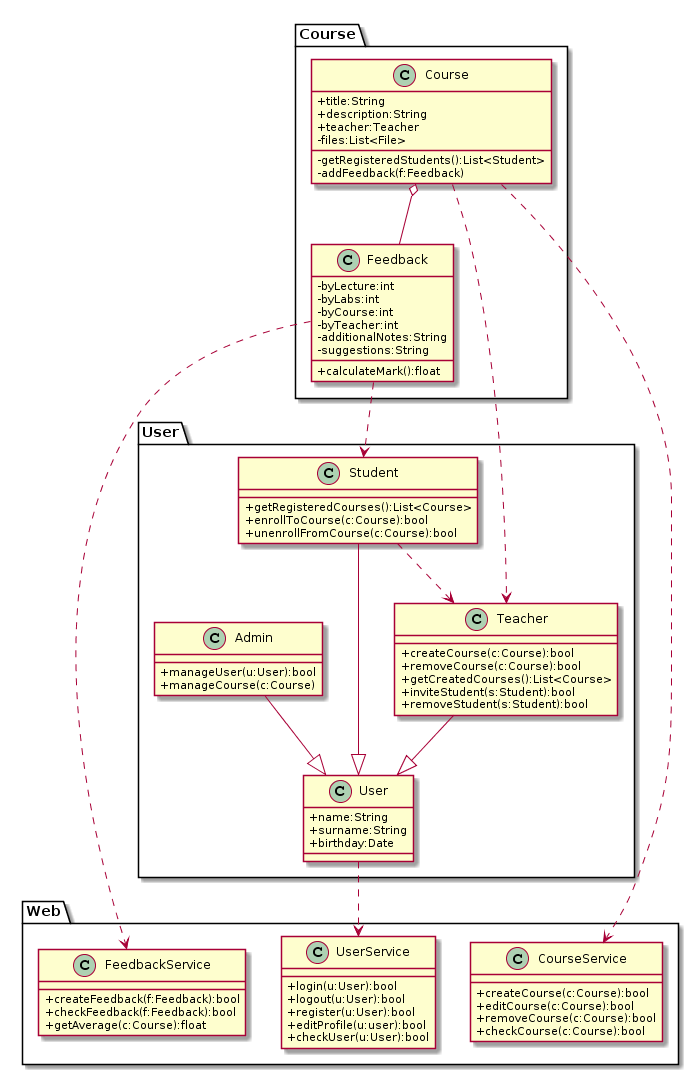
\includegraphics[width=15cm]{5class}
	\caption{Class diagram}
	\label{fig:5class}
\end{figure}
The diagram is divided in 3 packages: User, Web, Course. The "Course package" contains the classes Feedback and Course. Feedback is part of Course, that's why they are in agregation relationship. The "User" package contains 3 classses: Admin, Teacher and Student which inherit from the User class. The Feedback depends of Student. The Stdent depends of the Teacher (enroll/unenroll). Also the Course depends of the Teacher.\par
There is the third package, "Web". It includes FeedbackService, UserService and CourseService, each being a "dependee" for Feeback, User and Course classes respectively.

\subsection{Statechart Diagram}
In Figure ~\ref{fig:6userAccount} is represented the statechart diagram for the user account.
\begin{figure}[H]
\centering
	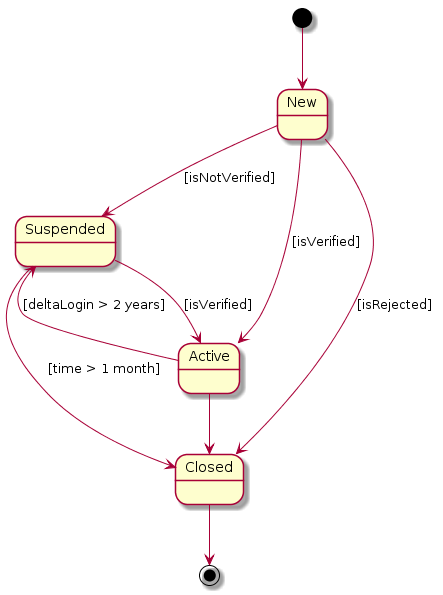
\includegraphics[width=10cm]{6userAccount}
	\caption{User account statechart diagram}
	\label{fig:6userAccount}
\end{figure}
Initially all accounts are new (initialization). Those who had valid usernames and passwords, receive a notification by mail. Other ones are rejected, then closed. If the user does not verify the account, it becomes suspended. Suspenden accounts can become active if are verified in less than a month, else they are also closed. An active account with an "Offline" status more than 2 years, becomes supended and receives a new mail notification. Closed accounts have the final state.

In Figure ~\ref{fig:6courses} is represented the statechart diagram for courses.
\begin{figure}[H]
\centering
	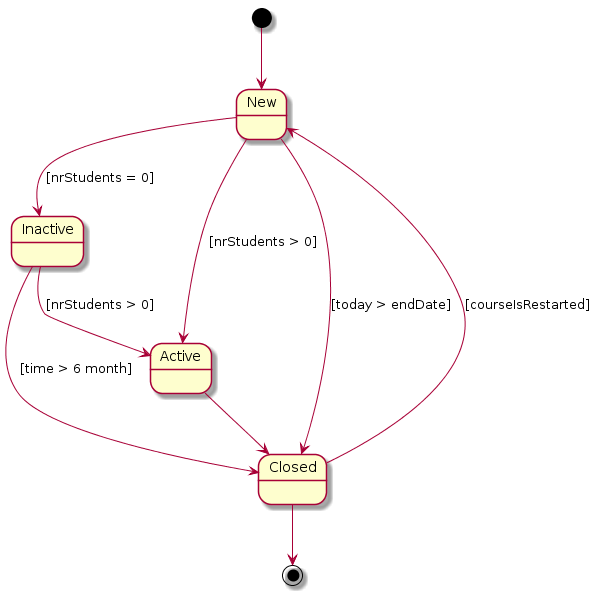
\includegraphics[width=10cm]{6courses}
	\caption{Courses statechart diagram}
	\label{fig:6courses}
\end{figure}
The teacher can create new courses. If he registers some users, the course becomes active. If there are no students at the beginning, the course is inactive. If he can't attract any students in half a year, the course is closed. If the starting date was incorect, the course is also closed. But any course can be restarted, if it was marked as closed.

In Figure ~\ref{fig:6search} is represented the statechart diagram for searching a course.
\begin{figure}[H]
\centering
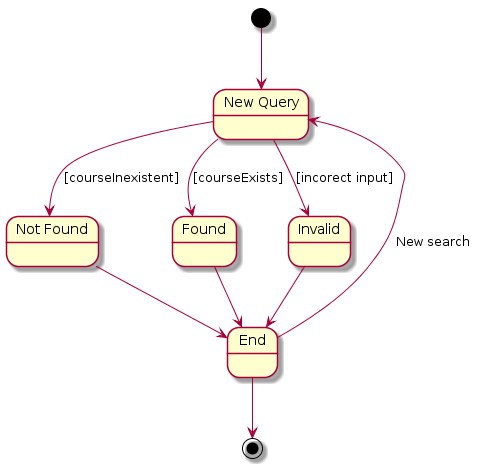
\includegraphics[width=10cm]{6search}
\caption{Search operation statechart diagram}
\label{fig:6search}
\end{figure}
An user who wants to search a course, creates a new query. If he inputs non-alfanumeric symbols, the result is invalidated. If the course is not found, the result is negative and a propper message appears. Otherwise, the course is found and a positive result with a success message is sent. All states then become finished.

\subsection{Activity Diagram}
In Figure ~\ref{fig:7login} is represented the activity diagram for user login.
\begin{figure}[H]
\centering
	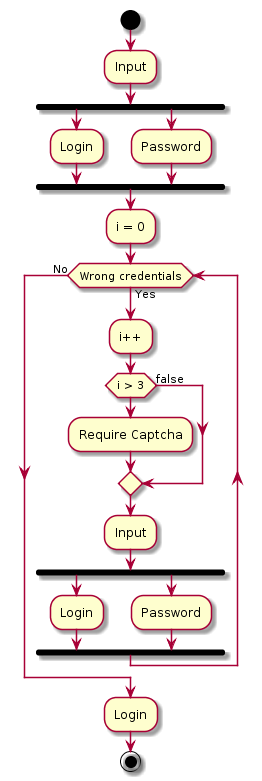
\includegraphics[width=5cm]{7login}
	\caption{Login activity diagram}
	\label{fig:7login}
\end{figure}
To login in an account, the user inputs login and password in any order. Then the input is submitted. If the credentials are right, the user is authenticated successfully. Otherwise, it should try again. If the third attempt is unsuccessful, he is requested to pass the captcha test. Any attempt from that moment will requre the additional test, until he inputs correct data.

\subsection{Component Diagram}
n Figure ~\ref{fig:8intermediar} is represented the component diagram for app, using the MVC pattern.
\begin{figure}[H]
\centering
	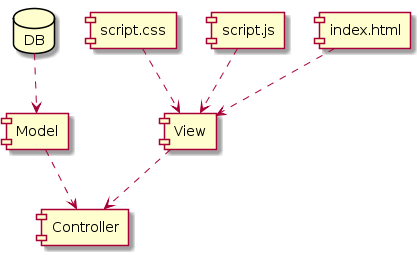
\includegraphics[width=10cm]{8intermediar}
	\caption{MVC component diagram}
	\label{fig:8intermediar}
\end{figure}
This is how the architecture of a MVC project looks like. The Model interacts with the database, but depends of the Controller. The View uses the controller to create the final products: .js and .css files which merge into the index.html.

In Figure ~\ref{fig:8final} is represented the component diagram for the app, after compiling, minifiing scripts.
\begin{figure}[H]
\centering
	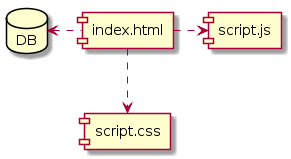
\includegraphics[width=10cm]{8final}
	\caption{Compiled files component diagram}
	\label{fig:8final}
\end{figure}
There is represented another step. After building the project, the final product is coposed by index.html file, a style, a scrip file and a database.

\subsection{Deployment Diagram}
In Figure ~\ref{fig:9deploy} is represented the deployment diagram for the app.
\begin{figure}[H]
\centering
	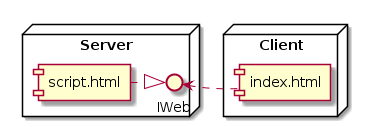
\includegraphics[width=10cm]{9deploy}
	\caption{Website deployment diagram}
	\label{fig:9deploy}
\end{figure}
The client node has an copy of the final product, provided by the internet. It depends of the interface realised by the server node application.\par

\section{Conclusion}
UML and Object-Oriented Modeling in general, plays a big role in software development. It forces you to think more abstract and approach OOP from an analytical point of view. Visual modeling creates an actual image of the future application. It produces abstract and accessible descriptions of both system requirements and designs. Also it decreases the "semantic gap" between the system and the real world. Then the system can be constructed using terminology that is almost the same as the non-technical personnel use in everyday business.\par
At first I had a problem with immagining an entire system. But when I started to build, diagram by diagram, studying every aspect of the project, the picture became clearer and clearer.
Also this work made us approach programming products from different sides: SWOT Analysis, Domain Analysis, Top-down and Bottom-up Design, Flow of Events etc.
The course achieved it's goal: to build a new set of skills which contribute to the evolution of a good software developer.

\begin{thebibliography}{9}
\bibitem{l1} 
Xiao He.
\textit{A metamodel for the notation of graphical modeling languages}, 2007.
\bibitem{l2} 
Omar El Gabry.
\textit{Object-Oriented Analysis And Design - Conceptual Model (Part 2)}, 2017.
\bibitem{l3} 
Stanislav Kozlovski.
\textit{A Short Overview of Object Oriented Software Design}, 2018.
\end{thebibliography}

\cleardoublepage

\end{document}
